%!TEX root = ./00_main.tex

\chapter{Scalability}
\label{sec:scalability}

In all of the previous experiments, only the 500 most prolific Twitter users in London were used. In the final experiment, this number of users is scaled up, by using 15,989 users that have a least two trajectories containing at least two observations each. Statistics for this data set are shown in Figure \ref{fig:15989_dist}. The quality of the observed trajectories is  much worse compared to the 500 most prolific users explored in Figure \ref{fig:500_dist}: In Figure \ref{fig:15989_traj} more than half of the trajectories have less than five trajectories within the twelve epochs, and only a small fraction of $6\%$ of the users have maximum number of twelve trajectories. In addition, Figure \ref{fig:15989_obs} shows the quality of these trajectories is much lower, as nearly $50\%$ of the trajectories have three or less observations. Due to the quality of this data a eight-fold split was no longer possible. A stratified shuffle split was used instead, taking 10 iterations of 20\% samples.

\begin{figure}[p]
	\centering
  \begin{subfigure}[b]{\textwidth}
    \centering
    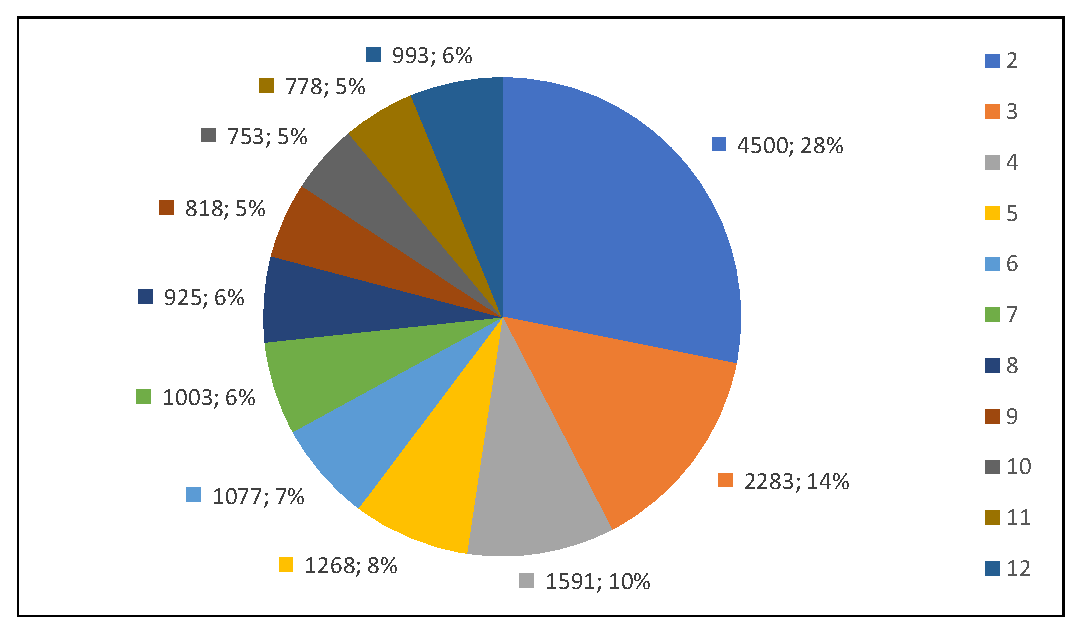
\includegraphics[width = 0.8\textwidth]{figures/15989_trajectories_per_user}
    \subcaption{Trajectories per user.}
    \label{fig:15989_traj}
  \end{subfigure}

  \begin{subfigure}[b]{\textwidth}
    \centering
    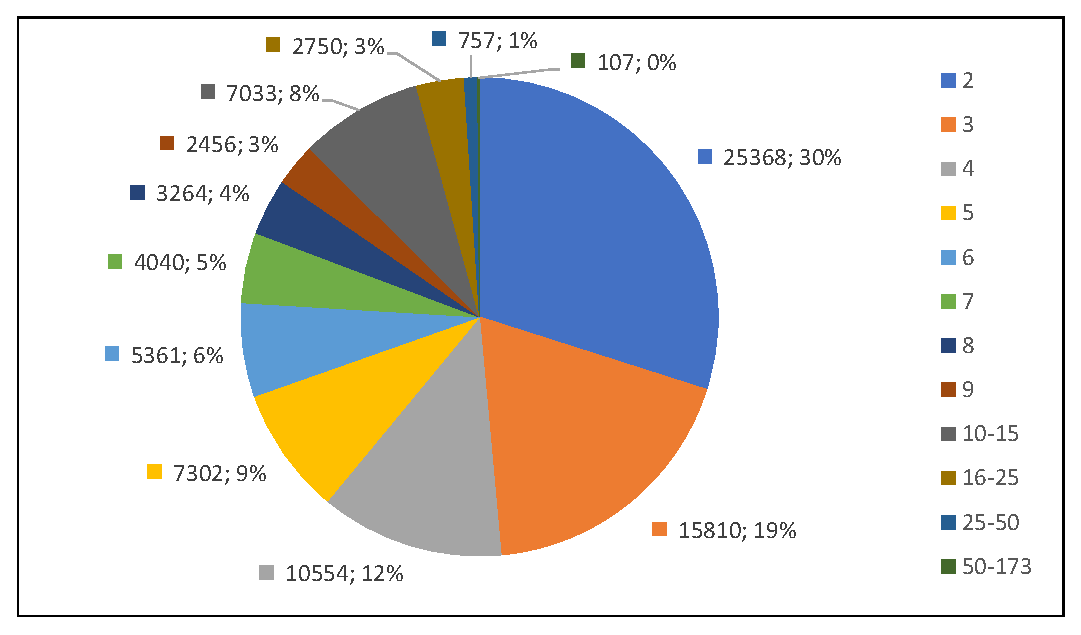
\includegraphics[width = 0.8\textwidth]{figures/15989_observations_per_trajectory}
  	\subcaption{Observations per one-week Trajectory}
    \label{fig:15989_obs}
  \end{subfigure}
  \caption{Distribution of all 15,989 users in the London-Twitter Dataset.}
  \label{fig:15989_dist}
	\figSpace
\end{figure}

The results on this data set, in terms of classification accuracy as well as run-times are shown in Figure \ref{fig:scalability_results}. In terms of accuracy, there is a vast decrease in accuracy observed, even for the default setting of $500$ users. This is because the experiments are no longer using the most prolific users, but just a random sample of users, and the data quality, in terms of number of observations per trajectory, as well as the number of trajectories per user, is much lower for these users.

\begin{figure}[p]
	\centering
  \begin{subfigure}[b]{\textwidth}
    \centering
    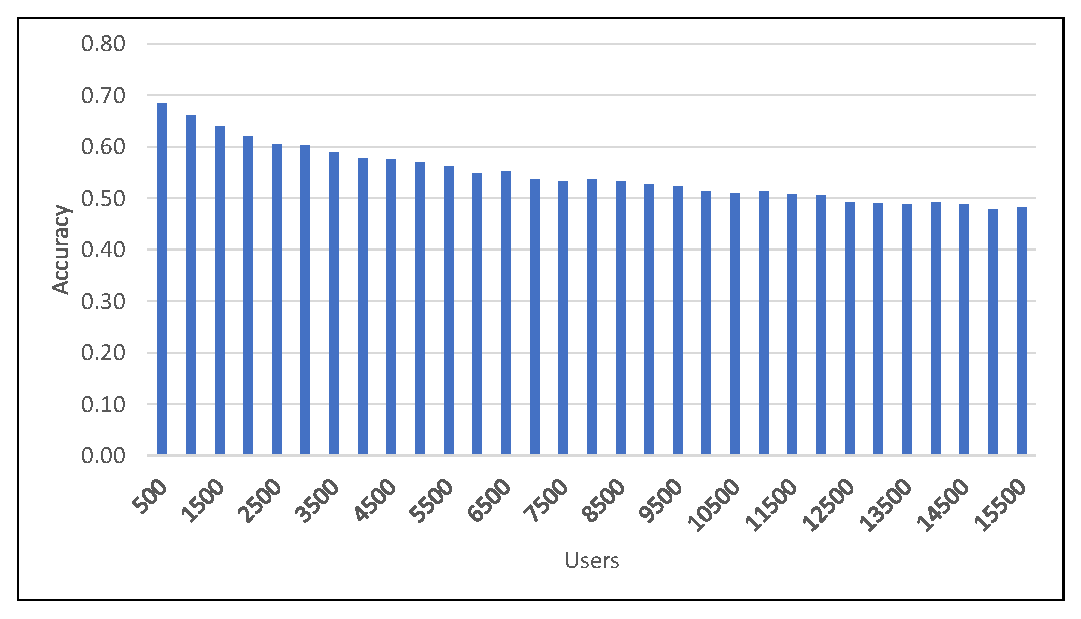
\includegraphics[width = 0.8\columnwidth]{figures/scalability_accuracy}
    \subcaption{Classification Accuracy}
    \label{fig:scalability_accuracy}
  \end{subfigure}

  \begin{subfigure}[b]{\textwidth}
    \centering
    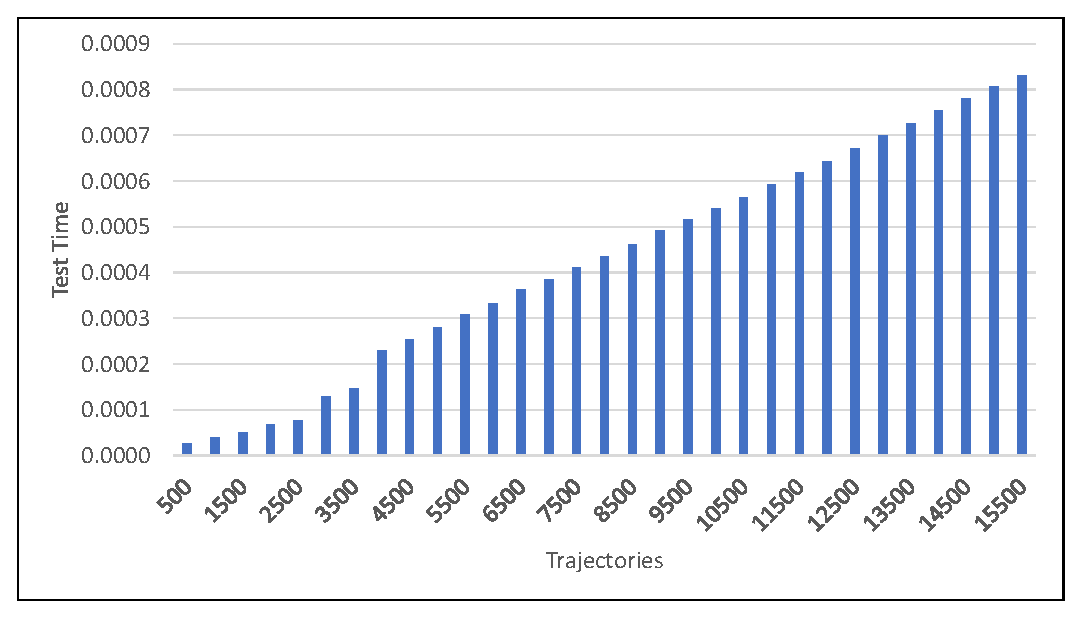
\includegraphics[width = 0.8\columnwidth]{figures/scalability_runtime}
    \subcaption{Run-time (in seconds)}
    \label{fig:scalability_runtime}
  \end{subfigure}
  \caption{Scalability: Scaling the number of Twitter users.}
  \label{fig:scalability_results}
	\figSpace
\end{figure}

Clearly, less prolific users are harder to classify, since there is less information. As the experiments are scaled up the number of users, there is a decrease in classification accuracy, as the classification problem becomes harder having more users. Still, the classification accuracy remains at almost $50\%$, despite the large number of  15,989 users, and the much lower trajectory quality.

Since a $k$NN classification is employed, and thus a lazy learning method is used, there is no model learning phase. The run-time results for the classification is shown in Figure \ref{fig:scalability_runtime}.\footnote{Run-time tests were performed on AWS using a m4.2xlarge EC2 instance running Amazon Linux. This instance type has 8 CPU cores and 32GB of RAM.} a linear run-time is observed, which is attributed to the extreme high dimensionality of the feature vectors, which cannot be beneficially supported by an index structure for the $k$NN search. But even at the full 15,989 users, the time to classify each trajectory is less than $1ms$.
